\section{Related Work on Pruning}
Pruning is the most widely studied form of model compression, and it has been applied to Transformers in a variety of ways. The related work discussion is organized along two coupled axes: the topology of the induced sparsity pattern and the optimization signal used to identify removable units. This framing keeps the deployment question explicit from the outset, because similar nominal compression ratios may correspond to different execution regimes, different preprocessing costs, and different forms of realized speedup.

\subsection{Problem Setting and Taxonomy}

\providecommand{\methoddetail}[1]{%
    \par\medskip
    \noindent{\bfseries #1}\par
    \smallskip\noindent
}
\providecommand{\methodsep}{%
    \par\smallskip
    \noindent\rule{0.28\textwidth}{0.35pt}
    \par\smallskip
}

Building on the formal framework introduced in Chapter~\ref{chap:neural_network_pruning}, the related-work discussion is organized along two coupled axes: the topology of the induced sparsity pattern and the optimization signal used to identify removable units.

\subsubsection{Taxonomy of Transformer Pruning Methods}

The main sparsity topologies were introduced formally in Section~\ref{sec:pruning_structures} (see Figure~\ref{fig:structures}). From a deployment standpoint, they differ in whether pruning yields compressed storage alone or native dense-shape acceleration after model surgery.

The taxonomy adopted here follows four coupled axes. The \emph{removable unit} determines whether the method acts on scalar weights or executable structures such as attention heads, FFN channels, and layers \cite{michel2022not,kurtic2022optimal}. The \emph{optimization signal} ranges from magnitude and activation statistics to differentiable mask learning, first-order Taylor criteria, second-order curvature surrogates, or search-based objectives \cite{sun2023simple,xia2022structured,ma2023llmpruner,frantar2023sparsegpt,kwon2022fast}. The \emph{recovery stage} distinguishes direct post-training pruning from methods requiring LoRA recovery, gradual fine-tuning, or distillation. The \emph{deployment objective} determines whether the reported benefit is compressed storage, dense-shape acceleration, or measured speedup \cite{kurtic2023ziplm,evopress2024,darwinlm2025}.

Each family corresponds to a different deployment objective. Unstructured methods such as Wanda and SparseGPT primarily optimize weight-level saliency \cite{sun2023simple,frantar2023sparsegpt}. Structured methods span differentiable mask-learning (CoFi), dependency-aware gradient methods (LLM-Pruner), Fisher-based post-training frameworks, and runtime-aware second-order methods (ZipLM) \cite{xia2022structured,ma2023llmpruner,kwon2022fast,kurtic2023ziplm}. Search-based methods such as EvoPress and DarwinLM treat pruning as configuration optimization under explicit budget or hardware constraints \cite{evopress2024,darwinlm2025}. Figure~\ref{fig:pruning_taxonomy} and Table~\ref{tab:pruning_taxonomy} summarize this organization.

\begin{figure}[p]
	\centering
	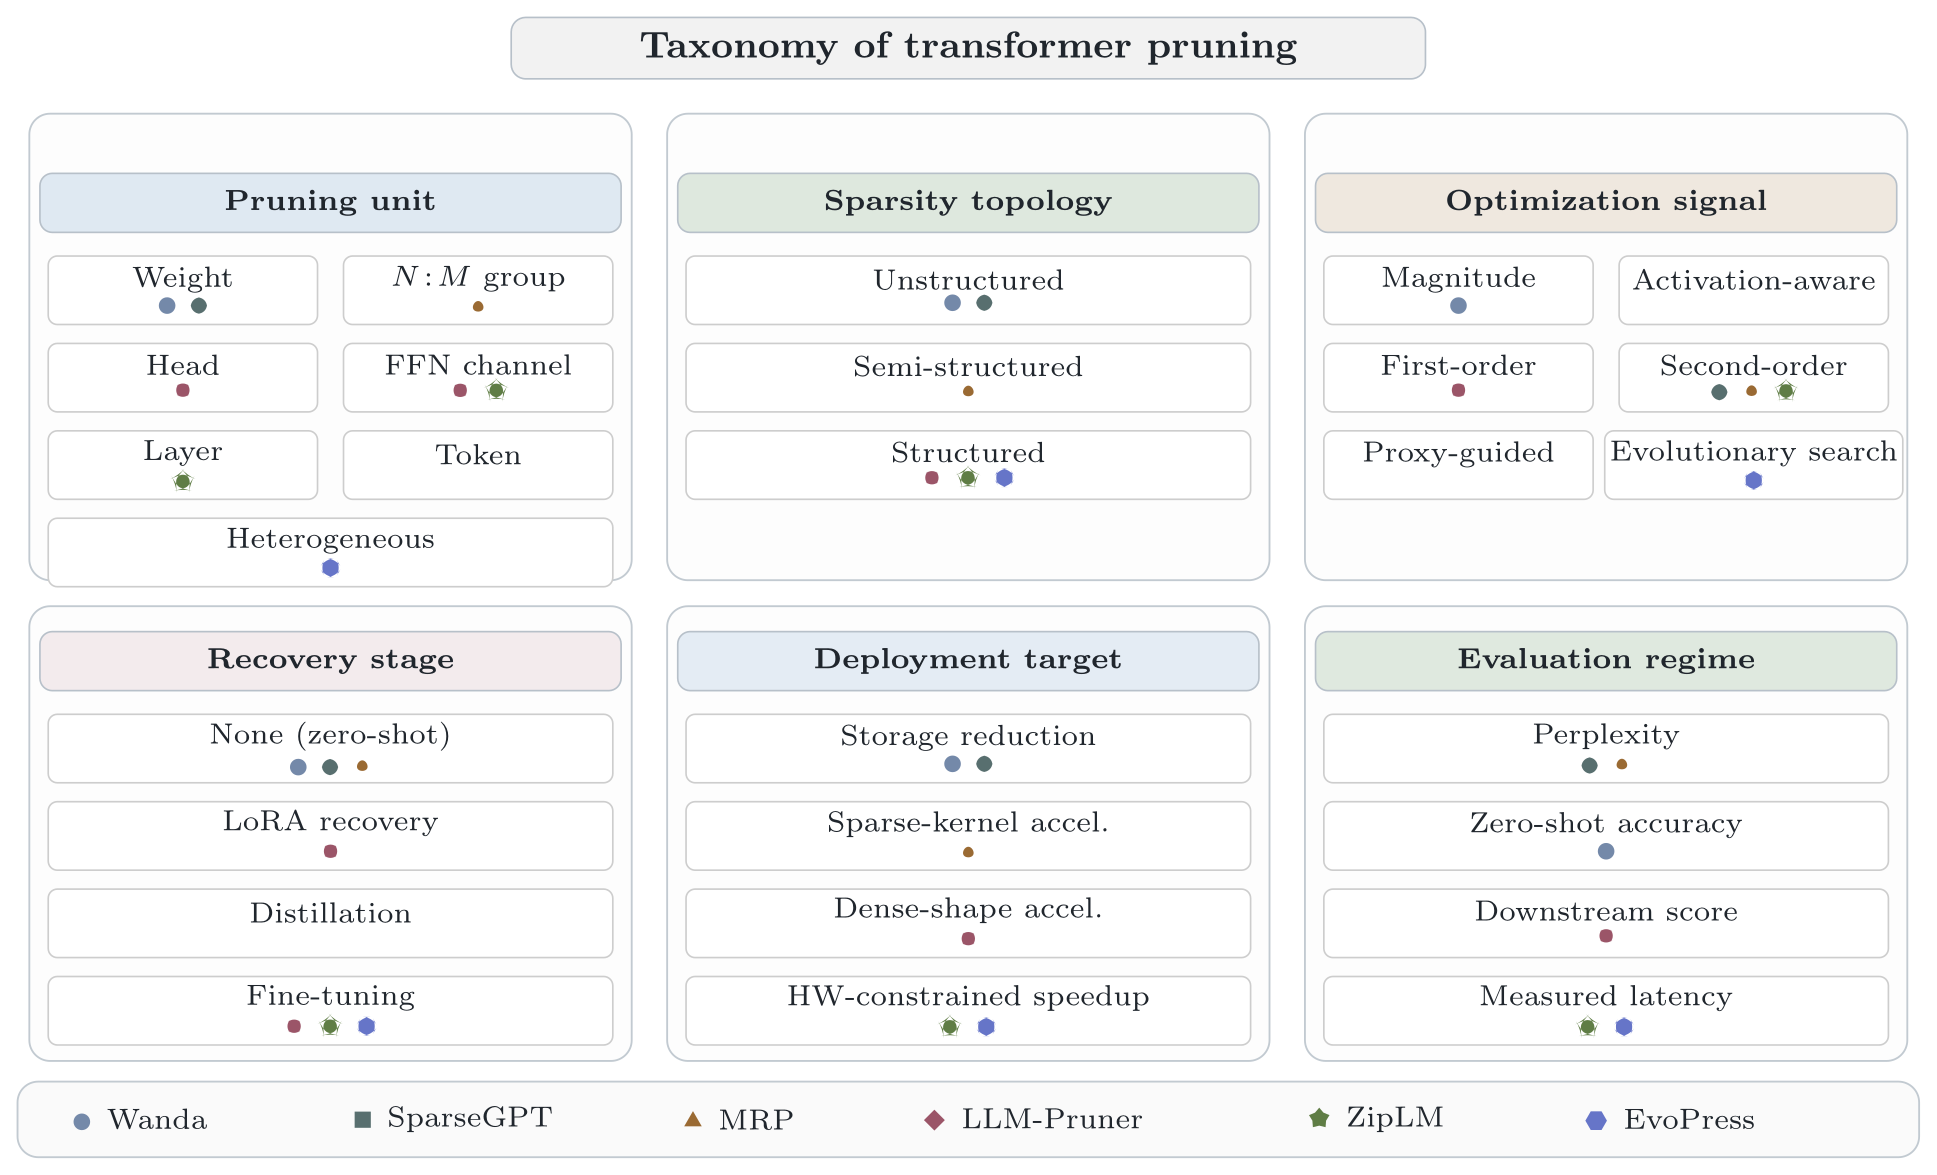
\includegraphics[width=\textwidth, height=0.88\textheight, keepaspectratio]{figures/compression/transformer_pruning_taxonomy.png}
	\caption{Taxonomy of the pruning methods considered in this chapter. The classification crosses the pruning unit, sparsity topology, optimization signal, recovery stage, deployment objective, and evaluation regime.}
	\label{fig:pruning_taxonomy}
\end{figure}

\begin{table}[H]
	\centering
	\caption{Taxonomy used to organize the pruning methods discussed in this chapter. The table distinguishes the removable unit, sparsity topology, optimization signal, recovery stage, and primary deployment claim for each method family.}
	\label{tab:pruning_taxonomy}
	\begin{tabularx}{\textwidth}{@{}l >{\raggedright\arraybackslash}X >{\raggedright\arraybackslash}X >{\raggedright\arraybackslash}X >{\raggedright\arraybackslash}X >{\raggedright\arraybackslash}X@{}}
		\toprule
		\textbf{Method} & \textbf{Unit} & \textbf{Topology} & \textbf{Signal} & \textbf{Recovery} & \textbf{Primary deployment claim} \\
		\midrule
		Wanda & Weight & Unstructured & Activation-aware saliency & None & Storage-oriented sparsity with strong zero-shot perplexity retention \\
		SparseGPT & Weight & Unstructured & Single-weight second-order compensation & None & High-sparsity pruning with local reconstruction \\
		CoFi & Layers / heads / FFN / hidden dimensions & Structured & Learned hard-concrete masks with $L_0$ control and distillation & Full task-specific pruning and fine-tuning & Dense-shape acceleration through jointly pruned Transformer structure \\
		LLM-Pruner & Heads / channels / blocks & Structured & First-order Taylor scoring with dependency groups & LoRA recovery & Structural compression with dense-shape execution \\
		Fast post-training pruning & Heads / FFN filters & Structured & Fisher-based constrained mask optimization & None beyond mask tuning & FLOPs- or latency-constrained structured pruning without retraining \\
		ZipLM & Heads / FFN dimensions & Structured & Second-order structured saliency with runtime-constrained search & Gradual fine-tuning and distillation & Measured speedup under device-specific constraints \\
		EvoPress / DarwinLM & Layer-wise compression levels & Heterogeneous structured & Proxy-guided or evolutionary search & Search-time evaluation or proxy training & Global configuration search under budget and hardware constraints \\
		\bottomrule
	\end{tabularx}
\end{table}

Figure~\ref{fig:pruning_taxonomy} should be read as a map of the chapter rather than as a ranking of methods. It separates the pruning literature by the kind of object being removed and by the signal used to decide removal. Table~\ref{tab:pruning_taxonomy} then makes this map concrete by assigning each reviewed method to a pruning unit, topology, scoring mechanism, recovery regime, and deployment claim.

The following subsections use this organization to review the selected pruning families in sequence: saliency-based methods, gradient-based structured methods, second-order methods, and search-based methods.

\clearpage
\subsection{Saliency-Based Methods}

Recall from Section~\ref{sec:pruning_criteria} that the Taylor expansion of the
loss change induced by pruning a weight $\theta_i$ produces a first-order term
proportional to the gradient and a second-order term capturing curvature
(Equation~\eqref{eq:taylor}). Saliency-based methods discard both terms and
instead use the weight magnitude or a proxy derived from activation statistics
as a surrogate for the true loss change. This zeroth-order approximation
requires no gradient computation and no calibration beyond a simple forward
pass, making these methods the cheapest option in the taxonomy.

\subsubsection{Magnitude and Activation-Aware Baselines}

\paragraph{Weight-Magnitude Pruning.}
Magnitude pruning uses absolute weight values as the saliency proxy:
\begin{equation}
	\mathcal{S}^{\mathrm{mag}}_{i,j} = |W_{i,j}|.
\end{equation}
Its core assumption is that small weights contribute less to the output and can be removed with limited degradation. The method requires no gradient-based recovery and remains the simplest baseline against which more sophisticated algorithms are evaluated.

\methodsep

\paragraph{Wanda (Weights $\times$ Activations).}
Wanda \cite{sun2023simple} refines this baseline by incorporating activation information from a small calibration set. The saliency score is
\begin{equation}
	\mathcal{S}^{\mathrm{wanda}}_{i,j} = |W_{i,j}| \cdot \|x_j\|_2,
\end{equation}
where $x_j$ is the $j$-th input activation channel and $\|x_j\|_2$ is its RMS norm estimated over $N$ calibration samples. The key insight is that importance is jointly encoded in weight magnitude and the energy of the coupled input channel.

\methoddetail{Algorithm Overview}
Both magnitude pruning and Wanda are one-shot post-training methods in the regime of Section~\ref{sec:post_training_pruning}: scores are computed once and no recovery training is applied afterward. Wanda processes each layer independently: it collects input activations on a small calibration set (typically 128 samples), computes per-weight saliency scores as the product of weight magnitude and activation norm, then prunes the lowest-scoring weights for each output neuron until the target sparsity $p$ is reached. No weight update or recovery step is applied. Magnitude pruning is a pure linear scan $O(|W|)$ with no calibration; Wanda adds only an activation-collection pass, keeping the overall cost near-linear.

These saliency methods are useful because they are cheap and easy to apply, but their decisions remain local. Once pruning moves from individual weights to heads, FFN channels, or layers, the method must account for structural dependencies between parameters. This motivates gradient-based structured pruning methods, where the score is computed over groups that can be removed consistently.

\subsection{Gradient-Based Methods}

Retaining the first-order term of the Taylor expansion (Equation~\eqref{eq:taylor}) gives a score proportional to the product of the gradient and the weight value. This makes the criterion sensitive to the direction of the loss landscape rather than just the weight magnitude, and it naturally extends to groups of weights by summing or aggregating the per-element scores. The methods in this section use exactly this first-order signal, applied to structured units such as heads, channels, and blocks rather than individual scalars.

Structured pruning replaces individual-weight saliency with group-level importance, because the natural units in a Transformer, namely attention heads, FFN channels, and entire layers, are coupled through residual pathways and shared projection matrices. Removing one head, for example, requires deleting consistent slices from $W_Q$, $W_K$, $W_V$, and $W_O$ together; removing an FFN channel removes coordinated rows and columns from the two projection matrices. Any pruning criterion applied at this level must therefore identify groups that can be removed as a unit without breaking the forward pass \cite{michel2022not,kurtic2022optimal}.

\paragraph{LLM-Pruner.}
LLM-Pruner \cite{ma2023llmpruner} addresses the dependency problem explicitly by constructing a graph over the neurons of the network. For neurons $N_i$ and $N_j$ with input set $\mathrm{In}(N)$ and output set $\mathrm{Out}(N)$, the graph encodes two rules:
\begin{align}
	N_j \in \mathrm{Out}(N_i) \wedge \deg^{-}(N_j)=1 &\implies N_j \text{ depends on } N_i, \label{eq:dep1}\\
	N_i \in \mathrm{In}(N_j) \wedge \deg^{+}(N_i)=1 &\implies N_i \text{ depends on } N_j. \label{eq:dep2}
\end{align}
Here $\deg^{-}(N_j)$ is the in-degree of $N_j$ (number of neurons feeding into it) and $\deg^{+}(N_i)$ is the out-degree of $N_i$. The transitive closure of these rules groups all coupled parameters into a single dependency group $\mathcal{G} = \{W_i\}_{i=1}^M$, which is the minimal unit that can be consistently removed.

Once groups are defined, each is scored using a first-order Taylor approximation of the loss increase over a small calibration set $\mathcal{D}$. The importance of a structure tensor $W_i$ is estimated as
\begin{equation}
	I_{W_i}
	\approx
	\left|
	\frac{\partial \mathcal{L}^{\top}(\mathcal{D})}{\partial W_i}W_i
	-\frac{1}{2}W_i^{\top}HW_i
	\right|,
	\label{eq:taylor-vector}
\end{equation}
where $H$ is the local Hessian. The first-order gradient is retained alongside the Hessian term because the calibration set is only a proxy for the pretraining distribution; discarding it would introduce bias. An element-wise variant replaces $H$ with a Fisher-diagonal approximation. Individual tensor scores within a group are aggregated by sum, product, max, or last-only operators, and groups with the lowest aggregate score are removed first.

LLM-Pruner sits between a post-training and a recovery regime: scoring is post-training and requires no gradient propagation through the full model, but the pruned network is then passed through a LoRA recovery stage in line with the iterative recovery approach of Section~\ref{subsec:iterative_pruning}. LoRA adapters \cite{hu2021lora} are inserted into all linear modules and fine-tuned for two epochs over roughly 50K samples. The low-rank factors are then merged back into the weight matrices, leaving no adapter overhead at inference time. The full scoring stage requires only 10 short calibration sequences, making the preprocessing cost modest relative to the recovery phase.

\methodsep

\paragraph{CoFi.}
CoFi \cite{xia2022structured} is the main structured-pruning example of the learnable-mask criteria introduced in Section~\ref{subsec:learnable_adaptive_criteria}. It places binary masks on attention blocks, heads, FFN blocks, intermediate channels, and the shared hidden dimension, then optimises these masks jointly with the task loss:
\begin{align}
	\mathrm{MHA}(X) &= z_{\mathrm{MHA}} \sum_{i=1}^{N_h} z_{\mathrm{head}}^{(i)} \,\mathrm{Att}\!\left(W_Q^{(i)},W_K^{(i)},W_V^{(i)},W_O^{(i)},X\right), \\
	\mathrm{FFN}(X) &= z_{\mathrm{FFN}}\, \mathrm{gelu}(XW_U)\,\mathrm{diag}(z_{\mathrm{int}})\,W_D,
\end{align}
where $N_h$ is the number of attention heads, $W_Q^{(i)}, W_K^{(i)}, W_V^{(i)}, W_O^{(i)}$ are the query, key, value, and output projection matrices of head $i$, and $W_U$, $W_D$ are the up- and down-projection matrices of the FFN. Each mask variable $z$ is relaxed to a continuous value during training using the hard-concrete distribution for $L_0$ regularisation, which allows gradients to flow through the mask. The training objective combines task loss with a distillation term and a Lagrangian sparsity constraint:
\begin{equation}
	\mathcal{L}_{\mathrm{prune}}
	=
	\mathcal{L}_{\mathrm{task}}
	+
	\mathcal{L}_{\mathrm{distil}}
	+
	\lambda_1(\hat s - s_0)
	+
	\lambda_2(\hat s - s_0)^2,
\end{equation}
where $s_0$ is the sparsity target and $\hat{s}$ is the expected sparsity under the current mask distribution. Because the masks at different granularities interact, CoFi can discover structured subnetworks that a simple per-group ranking would miss.

\methoddetail{Algorithm Overview}
CoFi is a training-time iterative method in the sense of Section~\ref{subsec:iterative_pruning}: mask decisions and weight updates are interleaved throughout training rather than applied once. A warm-up phase first stabilizes the model weights before mask learning begins, with the sparsity constraint applied softly. The main phase then jointly optimises masks and weights under the Lagrangian objective, progressively tightening the sparsity target toward $s_0$ over training. Once the target is reached, each continuous mask variable is thresholded against zero to produce a binary decision, and a final fine-tuning pass is run on the surviving subnetwork. Because masks at all granularities are trained simultaneously, the discovered subnetwork reflects cross-level interactions rather than independent per-unit decisions.

Gradient-based structured pruning improves the consistency of the removed units, but the score still depends on a local approximation of how removal affects the loss. When pruning becomes more aggressive, interactions among remaining and removed weights become more important. This leads to second-order methods, which use curvature information or local reconstruction objectives to compensate for the error introduced by pruning.

\subsection{Second-Order Methods}

The second-order term of the Taylor expansion (Equation~\eqref{eq:taylor})
captures the curvature of the loss around the current weights. Retaining this
term, rather than discarding it as saliency and gradient methods do, allows the
pruning criterion to account for how much a removal actually shifts the loss
given the local geometry of the loss landscape. As discussed in
Section~\ref{subsec:second_order_criteria}, this leads to the OBS framework,
where the optimal weight correction after a removal is derived from the inverse
Hessian. The methods in this section apply that same principle at the scale of
modern LLMs, recovering tractability by restricting the Hessian computation to
individual layers or column blocks.

\subsubsection{Optimal Brain Compression Formulation}

For a layer with weight matrix $\mathbf{W} \in \mathbb{R}^{d_{\text{out}} \times d_{\text{in}}}$ and calibration activations $\mathbf{X} \in \mathbb{R}^{d_{\text{in}} \times n}$, the layer-wise sparse reconstruction problem is
\begin{equation}
	\min_{\mathbf{W}^{\text{sparse}}}
	\|\mathbf{W}\mathbf{X} - \mathbf{W}^{\text{sparse}}\mathbf{X}\|_F^2
	\quad \text{s.t.} \quad
	\|\mathbf{W}^{\text{sparse}}\|_0 \leq (1-p)\, d_{\text{out}} d_{\text{in}},
\end{equation}
where $\|\cdot\|_F$ is the Frobenius norm, $\|\cdot\|_0$ counts the number of nonzero entries, and $p \in (0,1)$ is the target sparsity ratio. Using the empirical Hessian proxy $\mathbf{H} = \mathbf{X}\mathbf{X}^T / n$, this becomes a curvature-aware reconstruction problem whose solution depends on $\mathbf{H}^{-1}$ to redistribute pruning error across remaining weights. The methods that follow differ in how they instantiate this objective: SparseGPT removes one scalar weight at a time, MRP removes an entire N:M group jointly, Fisher-based pruning applies curvature scoring to structured masks, and ZipLM extends the same principle to executable Transformer structures under runtime constraints.

\subsubsection{Single-Weight Iterative Removal (SparseGPT)}

SparseGPT \cite{frantar2023sparsegpt} greedily prunes one weight at a time while applying compensation updates to remaining weights in the current block. This can be read as a blockwise version of the OBS correction introduced in Section~\ref{subsec:obd_obs} and formalised for large linear layers in Section~\ref{subsec:second_order_criteria}. Its local objective at iteration $t$ is
\begin{equation}\label{eq:srp}
	\min_{\delta w} \frac{1}{2}\delta w^T H \delta w
	\quad\text{s.t.}\quad
	(w+\delta w)\cdot e_t = 0,
\end{equation}
where $e_t$ is the one-hot selector for the pruned weight.

\methoddetail{Algorithm Overview}
SparseGPT is a post-training one-shot method in the regime of Section~\ref{sec:post_training_pruning}: pruning and compensation are applied in a single forward pass over the layers without any subsequent gradient-based recovery. It processes the weight matrix in column blocks of size $B$. For each block, it first constructs the regularized inverse Hessian $(XX^T + \lambda I)^{-1}$. Within each block, it iteratively identifies the weight with minimum local second-order loss, sets it to zero, then updates the remaining weights in that block using the corresponding column of $\mathbf{H}^{-1}$. After processing a block, lazy batch updates are applied to adjacent blocks. The method scales as $O(d_{\text{in}}^2 d_{\text{out}} + d_{\text{in}}^3/B)$ per layer, with a calibration budget of approximately 128 samples.

It is more instructive to understand SparseGPT as a weight-level, Hessian-compensated method for pruning: each decision to prune weights is made locally, and weights are updated to make the layer output's deviation as minimal as possible \cite{frantar2023sparsegpt}. It is through this same lens that SparseGPT's modification for semi-structured N:M sparsity can be understood, where the compensation method is kept and mask selection is constrained to local groups. If the block size is set to $B_s = M$, and from each group of $M$ weights the $N$ weights with the smallest OBS reconstruction score are selected for removal, the compensation becomes more localized to a block rather than the whole layer. Within that block, however, weights are still selected and compensated one at a time, so the compensation at each step does not account for the interactions among the other weights being simultaneously removed from the same group, which is the gap MRP directly addresses.

\methodsep

\subsubsection{Joint Optimization for Multi-Weight Removal (MRP)}

The MRP framework \cite{zhao2024pruning} generalizes second-order pruning to N:M groups. For a vectorized weight block $w$ and binary pruning mask $M$, where $M_i=1$ indicates that weight $i$ is pruned, the objective minimizes the second-order loss increase for the full group:
\begin{equation}\label{eq:ptp}
	\min_{\delta w} \frac{1}{2}\delta w^T H \delta w + g^T \delta w
	\quad\text{s.t.}\quad
	(w+\delta w)\odot M = 0,
\end{equation}
where $g$ is the gradient of the loss with respect to $w$, and $\odot$ denotes elementwise multiplication. Solving the group jointly yields a compensation update for the retained weights:
\begin{equation}
	\delta w^\star = -H_{\bar{M}\bar{M}}^{-1}(g_{\bar{M}} + H_{\bar{M}M}w_M),
\end{equation}
where $M$ denotes pruned indices, $\bar{M}$ retained indices, and $w_M$ the weight values at the pruned coordinates. This expression makes the role of the block Hessian explicit: in N:M pruning, the removed weights are not independent decisions, so compensation must be computed for the group rather than for a single scalar.

\methoddetail{Algorithm Overview}
MRP is a post-training one-shot method in the regime of Section~\ref{sec:post_training_pruning}: no gradient updates or recovery training are applied after pruning. It operates layer by layer. For each layer, the block Hessian is estimated from calibration activations. The weight tensor is partitioned into non-overlapping groups of $M$ consecutive weights. For each group, the joint second-order problem is solved: the mask selecting the $M-N$ weights with the highest reconstruction cost is identified, and the compensation update $\delta w^\star$ is applied to the retained $N$ weights before the next group is processed. Because the group is treated as a unit rather than a sequence of scalar removals, the method correctly accounts for interactions among simultaneously pruned coordinates within the block.

Figure~\ref{fig:hessian_compensation} illustrates this difference. SparseGPT compensates after removing one scalar weight, whereas MRP compensates after removing a constrained local group. The figure is therefore used to distinguish scalar second-order correction from group-level second-order correction.

\begin{figure}[H]
\centering
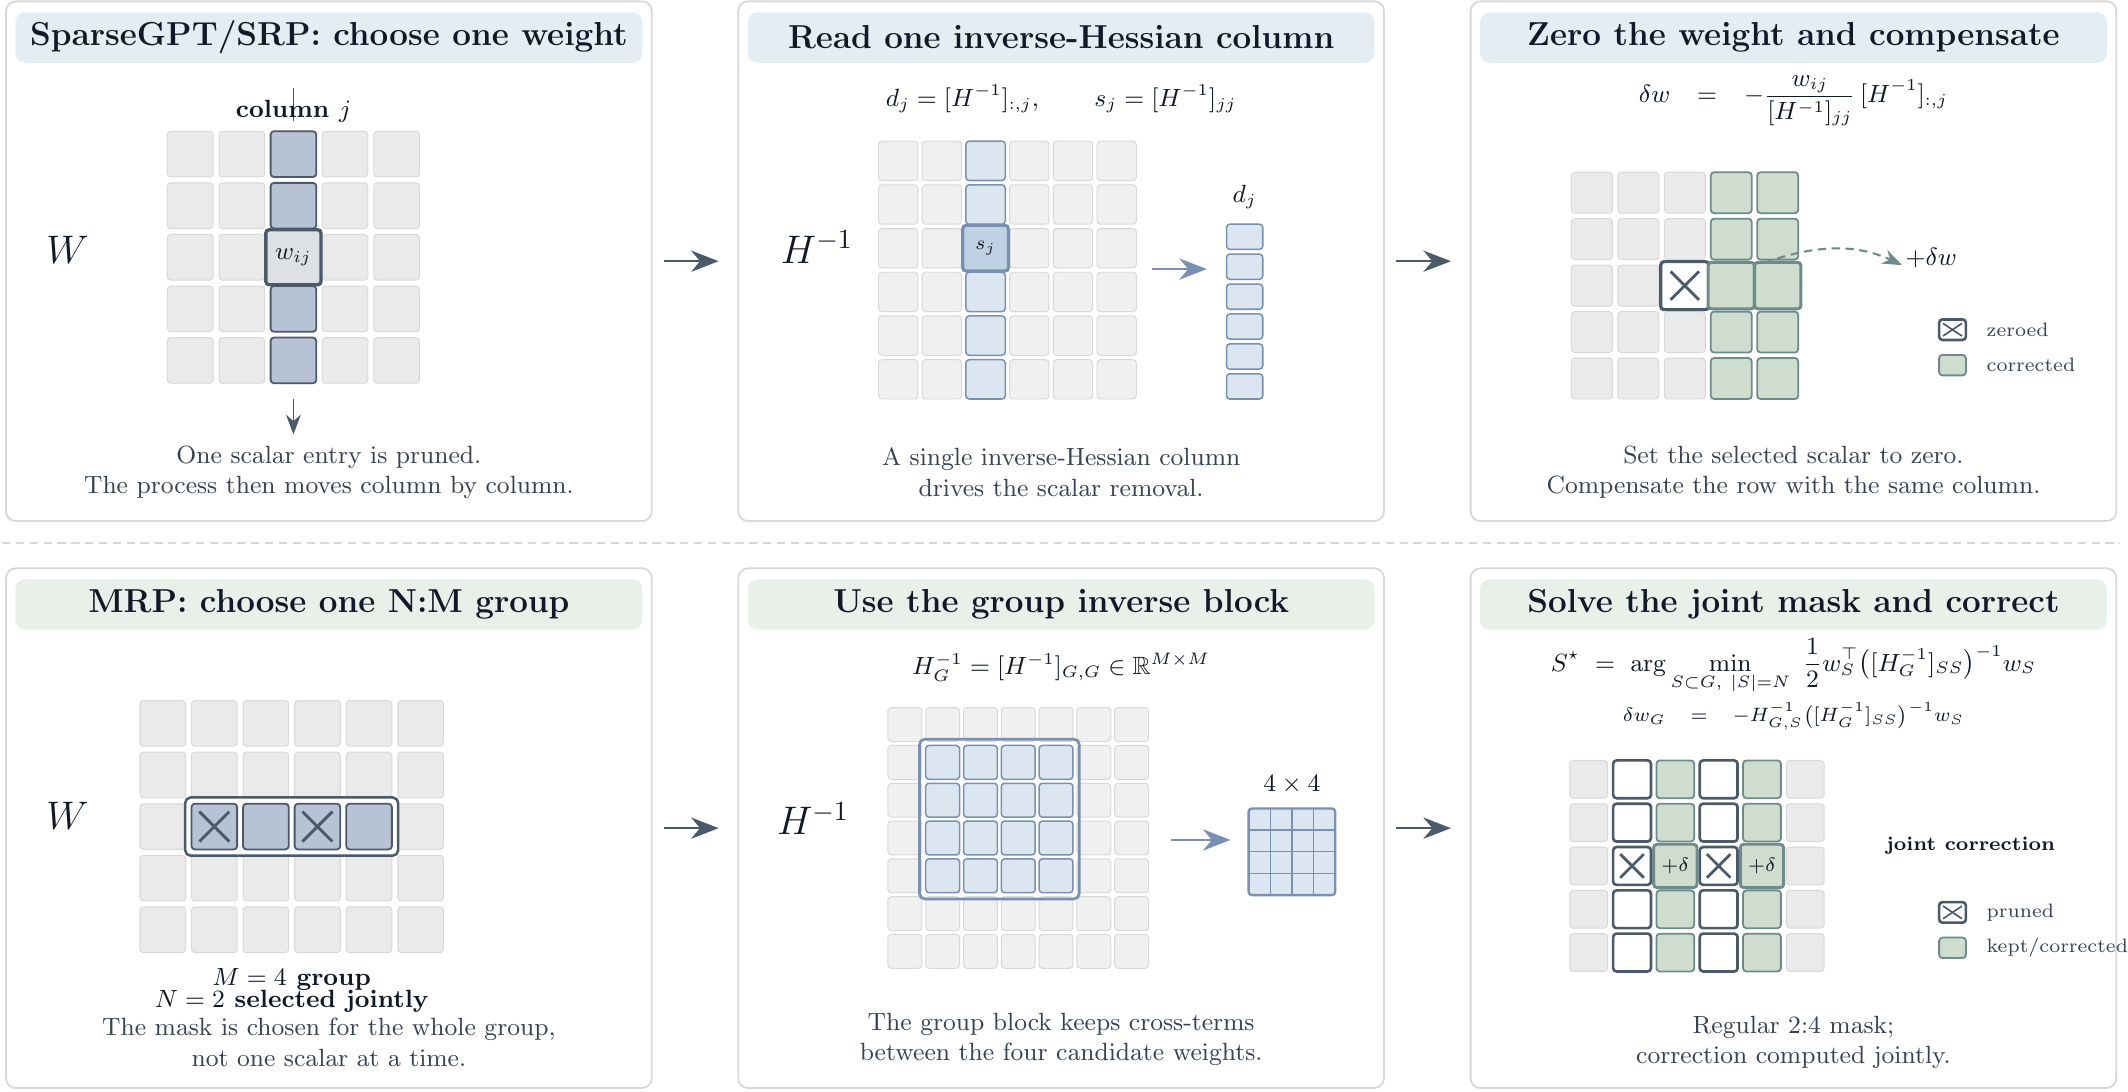
\includegraphics[width=\linewidth]{figures/compression/sparsegpt_mrp_compensation.png}
\caption{Second-order compensation strategies for unstructured and semi-structured pruning. SparseGPT removes one scalar weight per step and compensates using one column of $\hat{H}^{-1}$, while MRP removes an N:M group jointly and uses the block $(\hat{H}^{-1}_{MM})^{-1}$ to model interactions among simultaneously removed weights.}
\label{fig:hessian_compensation}
\end{figure}

\methodsep

\subsubsection{Fisher-Based Post-Training Structured Pruning}

The post-training framework of Kwon et al. \cite{kwon2022fast} applies second-order structured pruning without end-to-end post-pruning weight optimization. Binary masks over attention heads and FFN filters are found by solving
\begin{equation}
	\arg\min_{\mathbf{m}} \mathcal{L}(\mathbf{m})
	\quad \text{s.t.} \quad
	\mathrm{Cost}(\mathbf{m}) \leq C,
\end{equation}
where $\mathrm{Cost}$ is either a FLOPs or measured latency budget. Expanding around the dense mask and applying a diagonal Fisher approximation reduces the search to selecting units with the smallest diagonal Fisher scores subject to the cost constraint. For latency-constrained pruning, a piecewise-linear lookup table replaces the analytical cost model to incorporate real device behavior:
\begin{equation}
	\mathrm{LAT}(\mathbf{m}_{\ell}) =
	\begin{cases}
		0, & \|\mathbf{m}_{\ell}\|_0 = 0, \\
		c, & 0 < \|\mathbf{m}_{\ell}\|_0 \leq T, \\
		a(\|\mathbf{m}_{\ell}\|_0 - T) + c, & \|\mathbf{m}_{\ell}\|_0 > T,
	\end{cases}
\end{equation}
where $c$ is the base latency incurred by any non-empty layer configuration, $T$ is the structural threshold below which latency is approximately constant, and $a$ is the slope capturing how measured latency grows beyond that threshold. All three constants are read from device benchmarks rather than derived analytically.

\methoddetail{Algorithm Overview}
The method proceeds in four steps: (1) diagonal Fisher scores are computed for head and FFN-filter masks on a small calibration set (2K training examples); (2) a FLOPs- or latency-constrained mask search is solved under the diagonal Fisher objective; (3) a block-diagonal Fisher refinement is applied layer by layer to recover interactions ignored by the diagonal approximation; (4) surviving mask values are tuned by layer-wise linear least-squares reconstruction. Because only mask values are updated, the method avoids end-to-end weight retraining. The paper reports pruning times of 39 seconds on GLUE and 135 seconds on SQuAD, compared to 33 hours for CoFi on MNLI.

\methodsep

\subsubsection{Inference-Aware Structured Second-Order Pruning (ZipLM)}

ZipLM \cite{kurtic2023ziplm} applies an OBS-style reconstruction objective to executable Transformer structures rather than scalar weights. For a candidate structure $S$ with column mask $\mathbf{M}_S$, the removal score is
\begin{equation}
	\arg\min_S
	\sum_{i=1}^{d_{\text{row}}}
	\mathbf{W}_{i,\mathbf{M}_S}
	\left(\left(\mathbf{H}^{-1}\right)_{\mathbf{M}_S,\mathbf{M}_S}\right)^{-1}
	\mathbf{W}_{i,\mathbf{M}_S}^{T},
\end{equation}
where $d_{\text{row}}$ is the output dimension of the weight matrix and the sum aggregates the reconstruction cost across all output rows. After removing a structure, the exact compensation and Hessian update are applied through block Gaussian elimination, so that all subsequent saliency scores remain consistent with the already-pruned state.

\methoddetail{Inference-Aware Search}
ZipLM adds a device-level objective on top of the local second-order scoring. It benchmarks attention and FFN configurations on the target hardware and stores measured runtimes in a lookup table. The global search then minimizes layer-wise structural sensitivity subject to a real speed constraint $\sum_\ell \tau_{\ell,s_\ell} \leq T_{\text{target}}$.

\methoddetail{Algorithm Overview}
ZipLM follows an iterative pruning-and-recovery regime in the sense of Section~\ref{subsec:iterative_pruning}: pruning steps are interleaved with fine-tuning rounds rather than applied all at once. It operates in two phases (see Figure~\ref{fig:ziplm_pipeline}). In the global phase, attention-head and FFN configurations are benchmarked on the target environment and a layer-wise sparsity profile satisfying the speedup requirement is selected. In the local phase, each selected layer is compressed by iteratively scoring candidate structures with the structured saliency metric, applying the optimal weight compensation, and updating the inverse Hessian by block Gaussian elimination. Recovery follows a gradual prune-and-fine-tune schedule with combined task, logit, and token-level distillation losses, at a cost of 8--10 fine-tuning epochs per pruning step.

\begin{figure}[H]
	\centering
	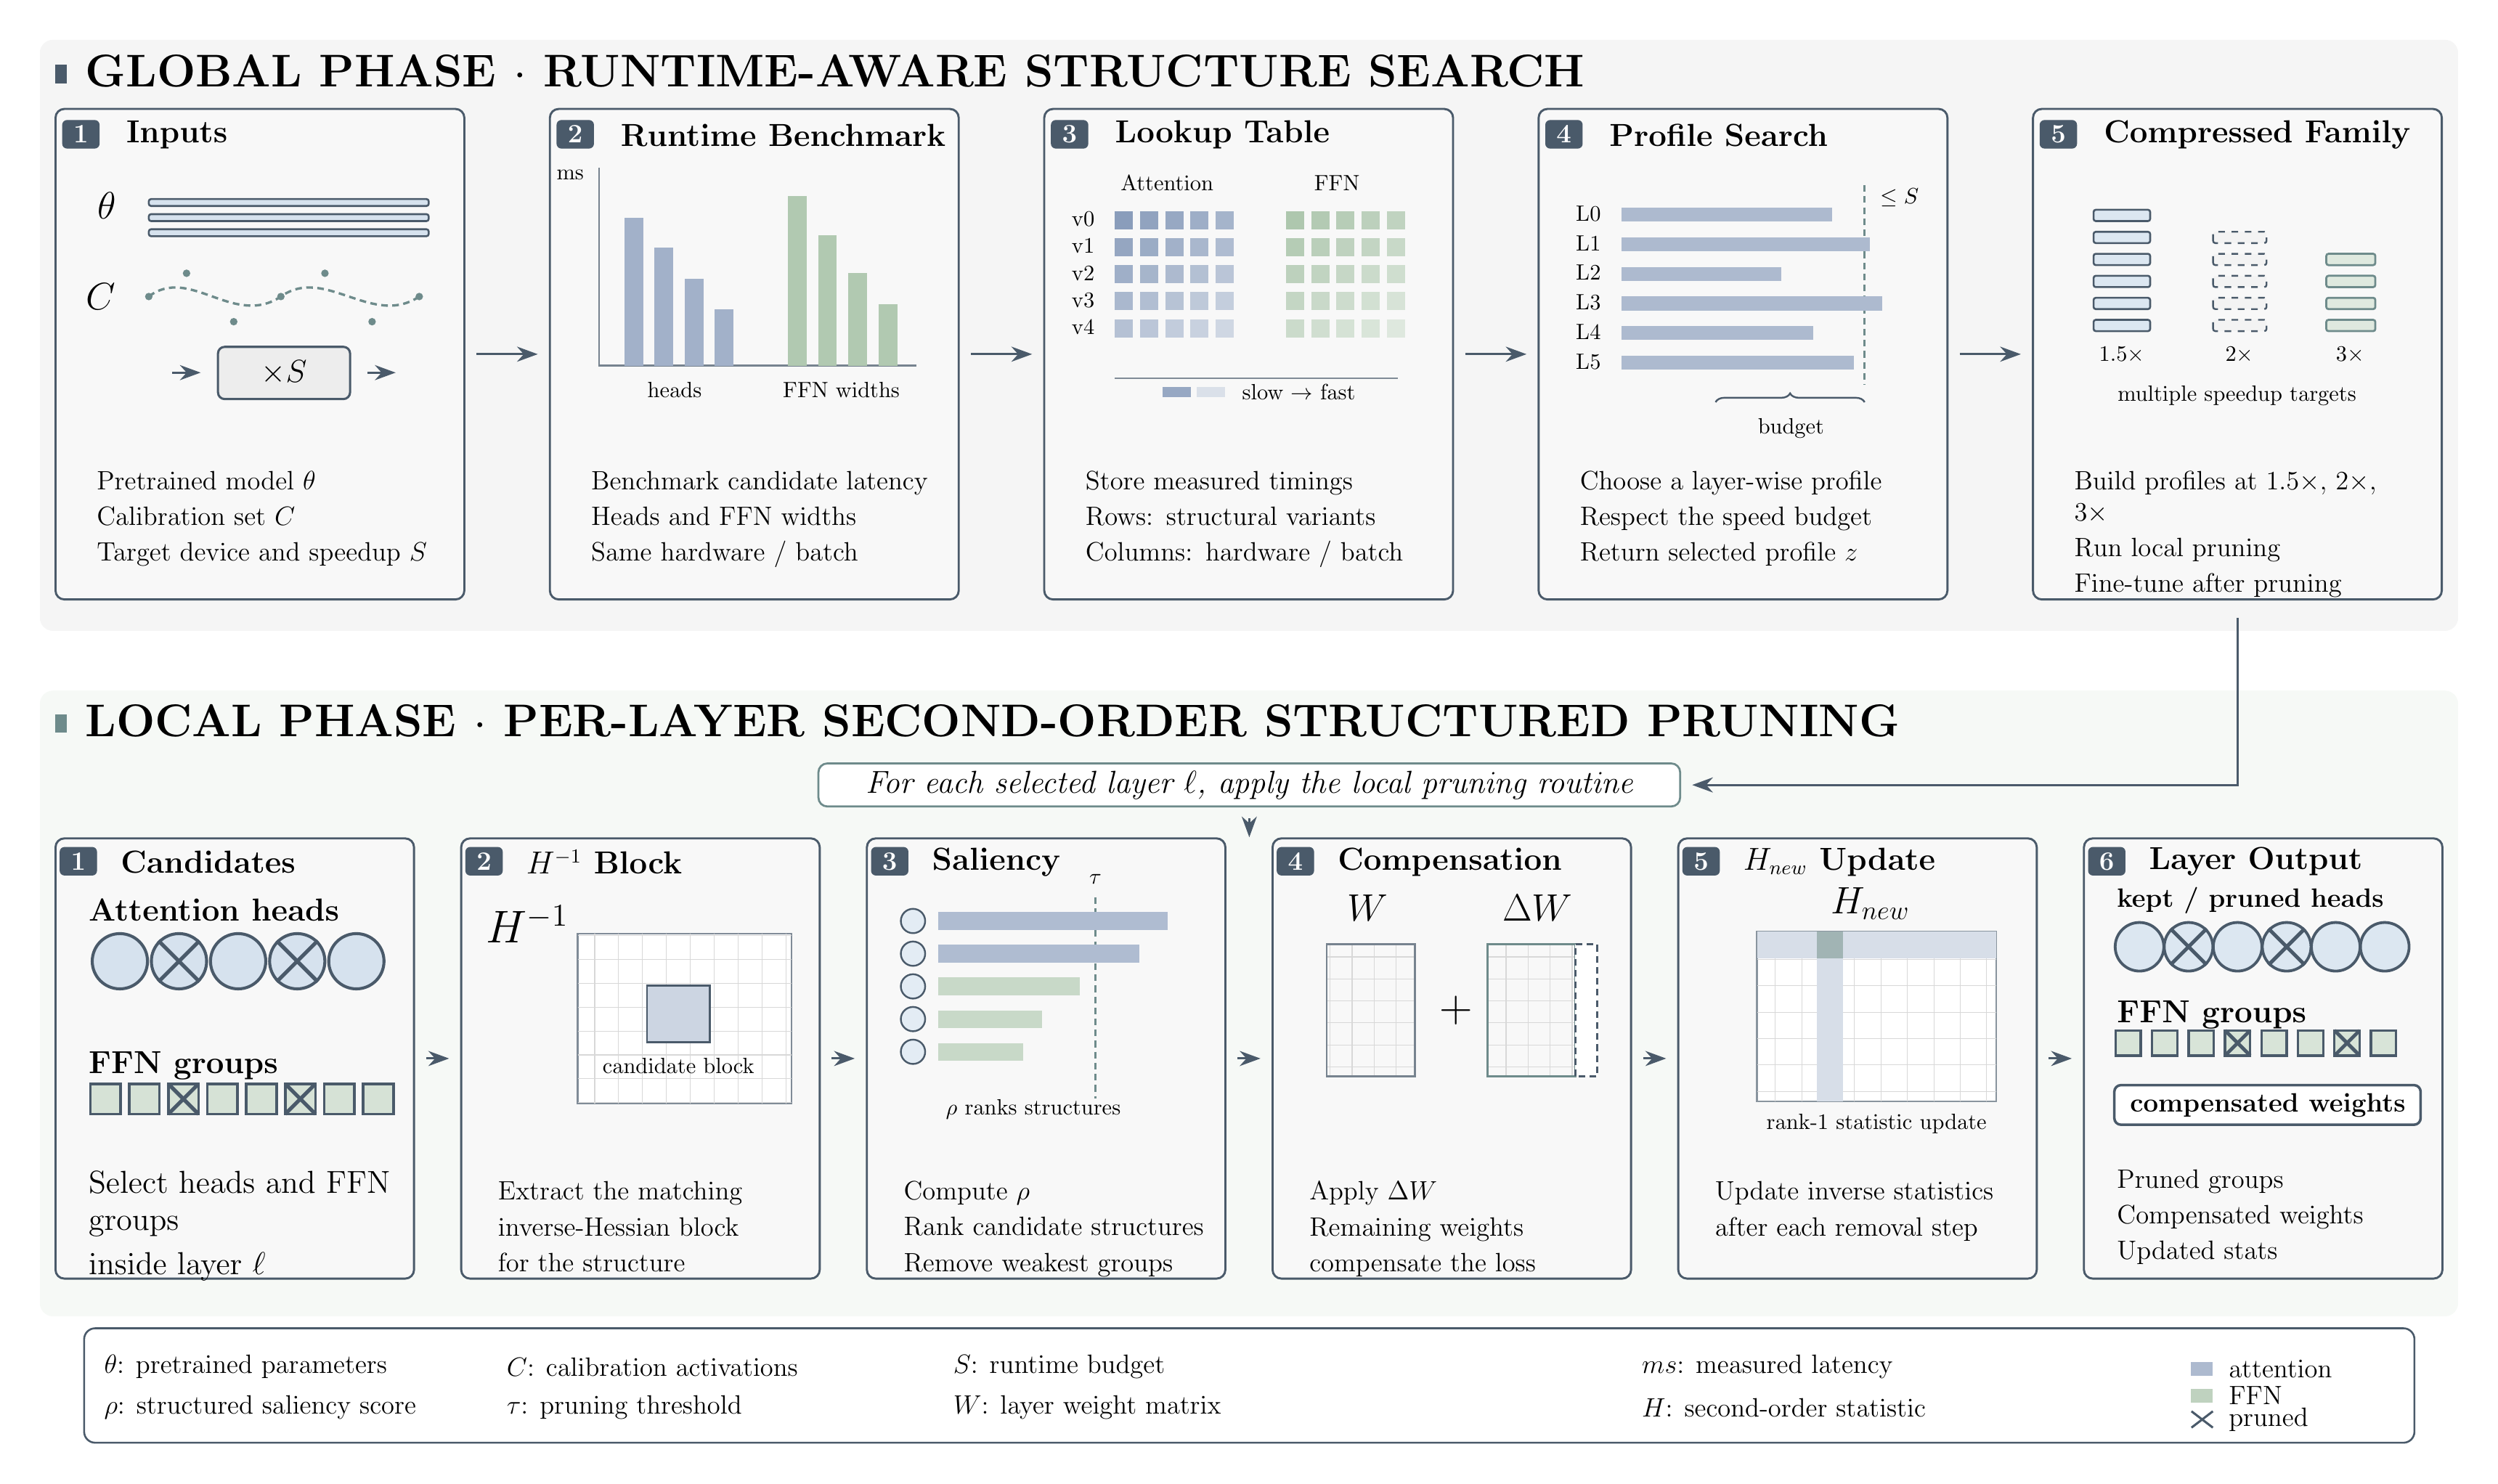
\includegraphics[width=0.96\textwidth]{figures/compression/ziplm_diagram.png}
	\caption{ZipLM pipeline. The global phase benchmarks attention-head and FFN configurations and searches for layer-wise sparsity profiles satisfying the required speedup. The local phase applies second-order structured pruning through inverse-Hessian scoring, compensation updates, and iterative Hessian refinement.}
	\label{fig:ziplm_pipeline}
\end{figure}

Second-order methods reduce local reconstruction error, but they do not fully resolve the allocation problem across the whole model. A method may know how to remove a head or channel with limited local damage and still not know how many heads or FFN channels should remain in each layer under a global budget. This is the point at which search-based methods become relevant.

\subsection{Search-Based Methods}

Search-based methods operate over complete sparsity configurations rather than applying a single closed-form ranking rule to individual units. This is especially relevant when the quality of a pruning decision depends on how several removals interact across layers.

\subsubsection{Constrained Evolutionary Frameworks}
\label{subsec:evopress_pruning}

\paragraph{EvoPress.}
EvoPress \cite{evopress2024} searches over discrete layer-wise compression profiles instead of assigning a single saliency score per layer. A candidate is a configuration $\mathbf{C} = \{c_1,\dots,c_L\}$ where $c_\ell \in \mathcal{S}_\ell$ is the compression level for layer $\ell$. Budget is preserved by level-switch mutation: one layer becomes more compressed only if another becomes less compressed, keeping the global average sparsity $S_{\text{glob}}$ fixed. Mutations are deliberately local, with most offspring differing from the parent by only one or two switches.

Selection proceeds in multiple rounds with increasing token budgets and decreasing survivor counts:
\begin{equation}
	\mathcal{P}^{(r+1)} =
	\operatorname{Top}_{n_{r+1}}
	\left(
	\left\{
	\mathcal{F}_{T_r}(C) \mid C \in \mathcal{P}^{(r)}
	\right\}
	\right),
	\qquad
	T_1<T_2<\cdots,\;
	n_1>n_2>\cdots,
\end{equation}
where the fitness signal is KL divergence to the reference model. This progressive evaluation scheme is what makes EvoPress practically efficient: early rounds use few tokens to discard poor candidates quickly, reserving the full calibration budget for finalists. The method converges in approximately 5--6 GPU hours for a standard Llama-2-7B sparsity search.

Figure~\ref{fig:evolutionary_pruning_flow} summarizes this search loop. The important point is that the algorithm evaluates complete compression profiles, selects promising candidates with increasing evaluation budgets, and mutates the retained profile while preserving the global compression constraint.

\begin{figure}[H]
\centering
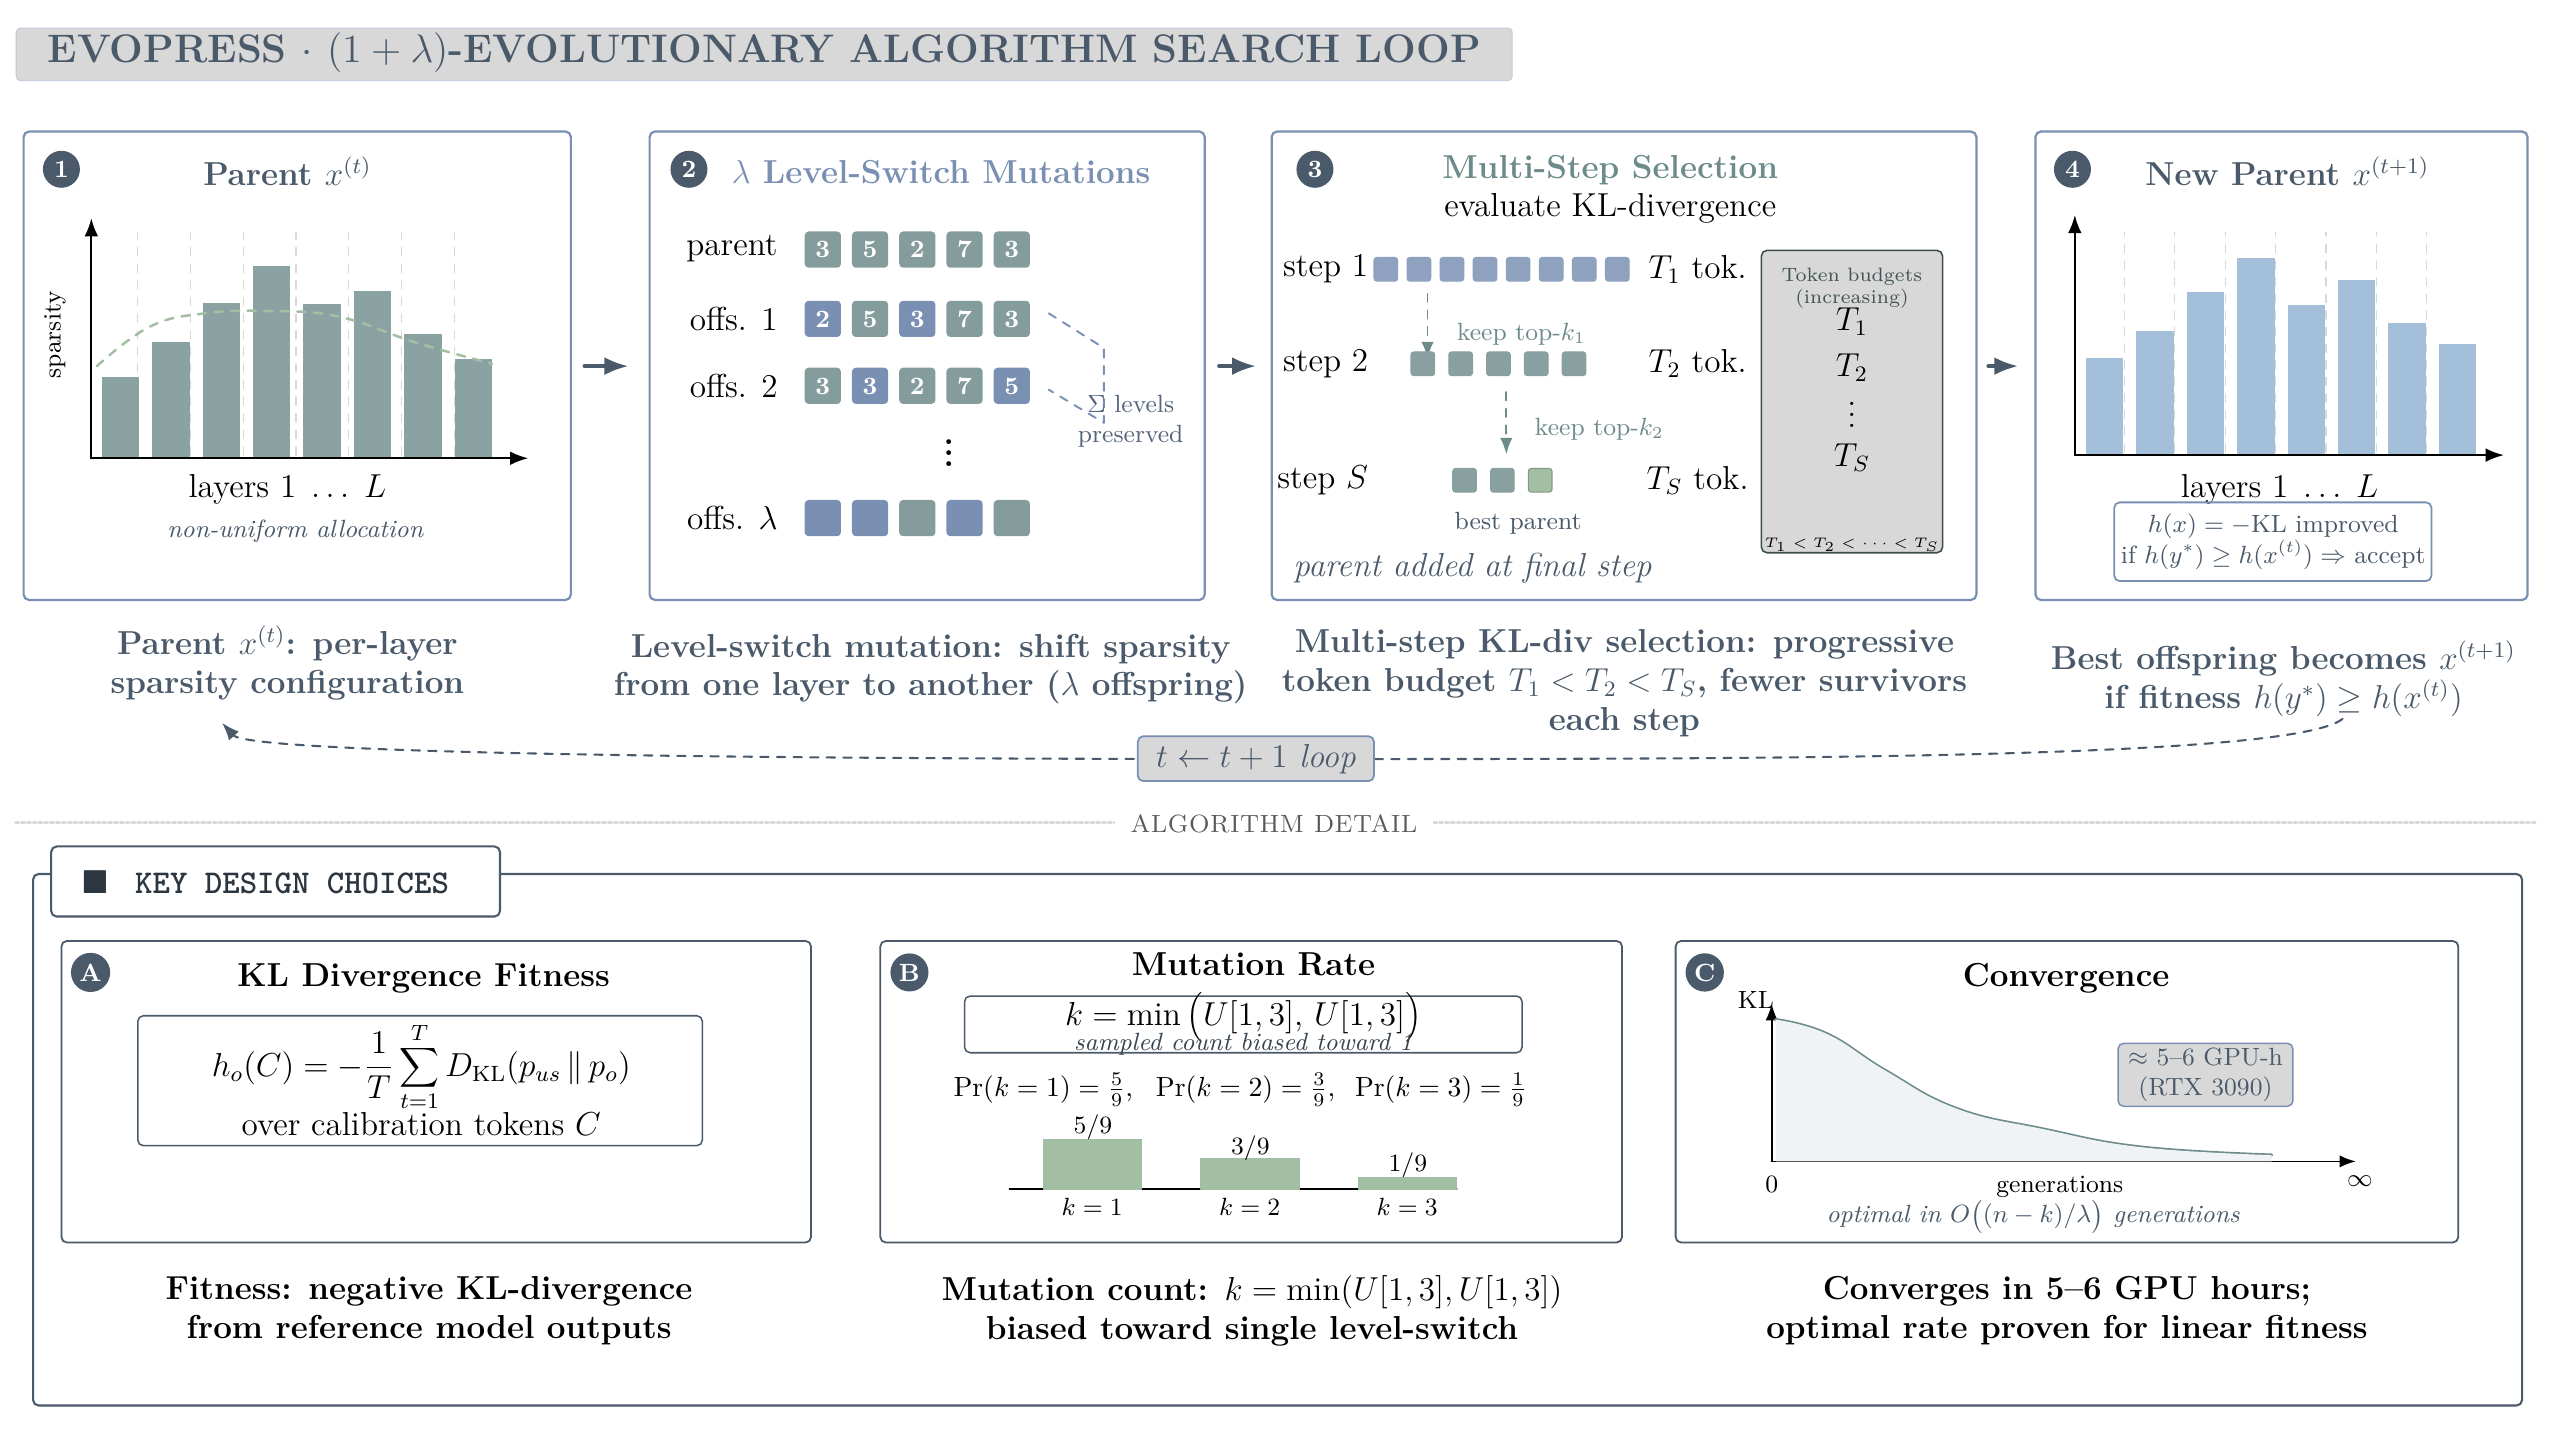
\includegraphics[width=0.94\linewidth,height=0.50\textheight,keepaspectratio]{figures/compression/evopress_search_loop.png}
\caption{EvoPress $(1+\lambda)$ evolutionary search loop for dynamic LLM compression \citep{evopress2024}. The method applies budget-preserving level-switch mutation and progressively evaluates candidates with larger calibration budgets.}
\label{fig:evolutionary_pruning_flow}
\end{figure}
\FloatBarrier

\methodsep

\paragraph{DarwinLM.}
DarwinLM \cite{darwinlm2025} extends evolutionary search to \emph{structured} pruning by unifying OBS-style second-order pruning with a training-aware offspring selection strategy. It differs from EvoPress on three axes: structured granularity (heads and FFN channels), front-loaded Hessian computation stored in a sparsity-level database (SLD), and fitness measured after a short lightweight finetune rather than from the one-shot pruned model.

\methoddetail{Sparsity Level Database}
For each module, DarwinLM solves the structured OBS problem at $N_l$ equally-spaced sparsity levels and stores the pruned-and-compensated weights. The optimal structured mask and compensation are:
\begin{align}
	M^* &= \arg\min_{M}\sum_{i=1}^{d_{\mathrm{row}}}
		\mathbf{W}_{i,M}\bigl(\hat{H}^{-1}_{MM}\bigr)^{-1}\mathbf{W}_{i,M}^\top, \\
	\delta^* &= -\mathbf{W}_{:,M}\bigl(\hat{H}^{-1}_{MM}\bigr)^{-1}\hat{H}^{-1}_{M,:},
\end{align}
where $d_{\mathrm{row}}$ is the output dimension of the module weight matrix, $M$ indexes the pruned columns, and $\hat{H}$ is the empirical Hessian computed from calibration activations. During search, candidate models are assembled by looking up stored entries, avoiding any Hessian recomputation.

\methoddetail{Training-Aware Selection}
Each candidate receives a short lightweight finetune before evaluation:
\begin{equation}
	\mathcal{F}(C_k) = D_{\mathrm{KL}}\!\bigl(\hat{M}\,\|\,\operatorname{finetune}(C_k,\, T_f)\bigr),
\end{equation}
where $\hat{M}$ is the output distribution of the dense reference model and $T_f$ is the fine-tuning token budget. Selection uses three progressive rounds ($T_f \in \{10\text{K}, 50\text{K}, 200\text{K}\}$ tokens) with decreasing survivor counts. The SLD must be computed once per model and sparsity range, making the upfront cost proportional to $L \cdot N_l$ structured OBS operations. DarwinLM compresses Llama-2-7B to 2.7B parameters with higher downstream accuracy than ShearedLlama using $5\times$ fewer post-training tokens (10B vs.\ 50B).

\methoddetail{Algorithm Overview}
DarwinLM sits between a post-training and an iterative regime: the SLD is built offline without end-to-end training, but each search candidate receives a lightweight fine-tune before fitness evaluation. In the offline phase, the SLD is built: for each module and each of $N_l$ sparsity levels, the structured OBS problem is solved and the pruned-and-compensated weights are stored, so that any candidate configuration can be assembled by table lookup rather than recomputation. In the search phase, candidate models are stitched together by selecting one SLD entry per module, then evaluated through that lightweight finetune. Mutation follows the same budget-preserving logic as EvoPress, swapping one module's sparsity level up only if another's is swapped down. Selection proceeds over three rounds with token budgets of 10K, 50K, and 200K and shrinking survivor counts, so weaker candidates are eliminated cheaply before the full evaluation budget is spent. The upfront SLD cost is proportional to $L \cdot N_l$ structured OBS operations and is paid once per model.

Figure~\ref{fig:darwinlm_pruning_flow} shows the corresponding DarwinLM workflow. Compared with EvoPress, the key visual distinction is the front-loaded sparsity-level database: candidate models are assembled from stored structured-pruning choices, then filtered through training-aware selection.

\begin{figure}[H]
\centering
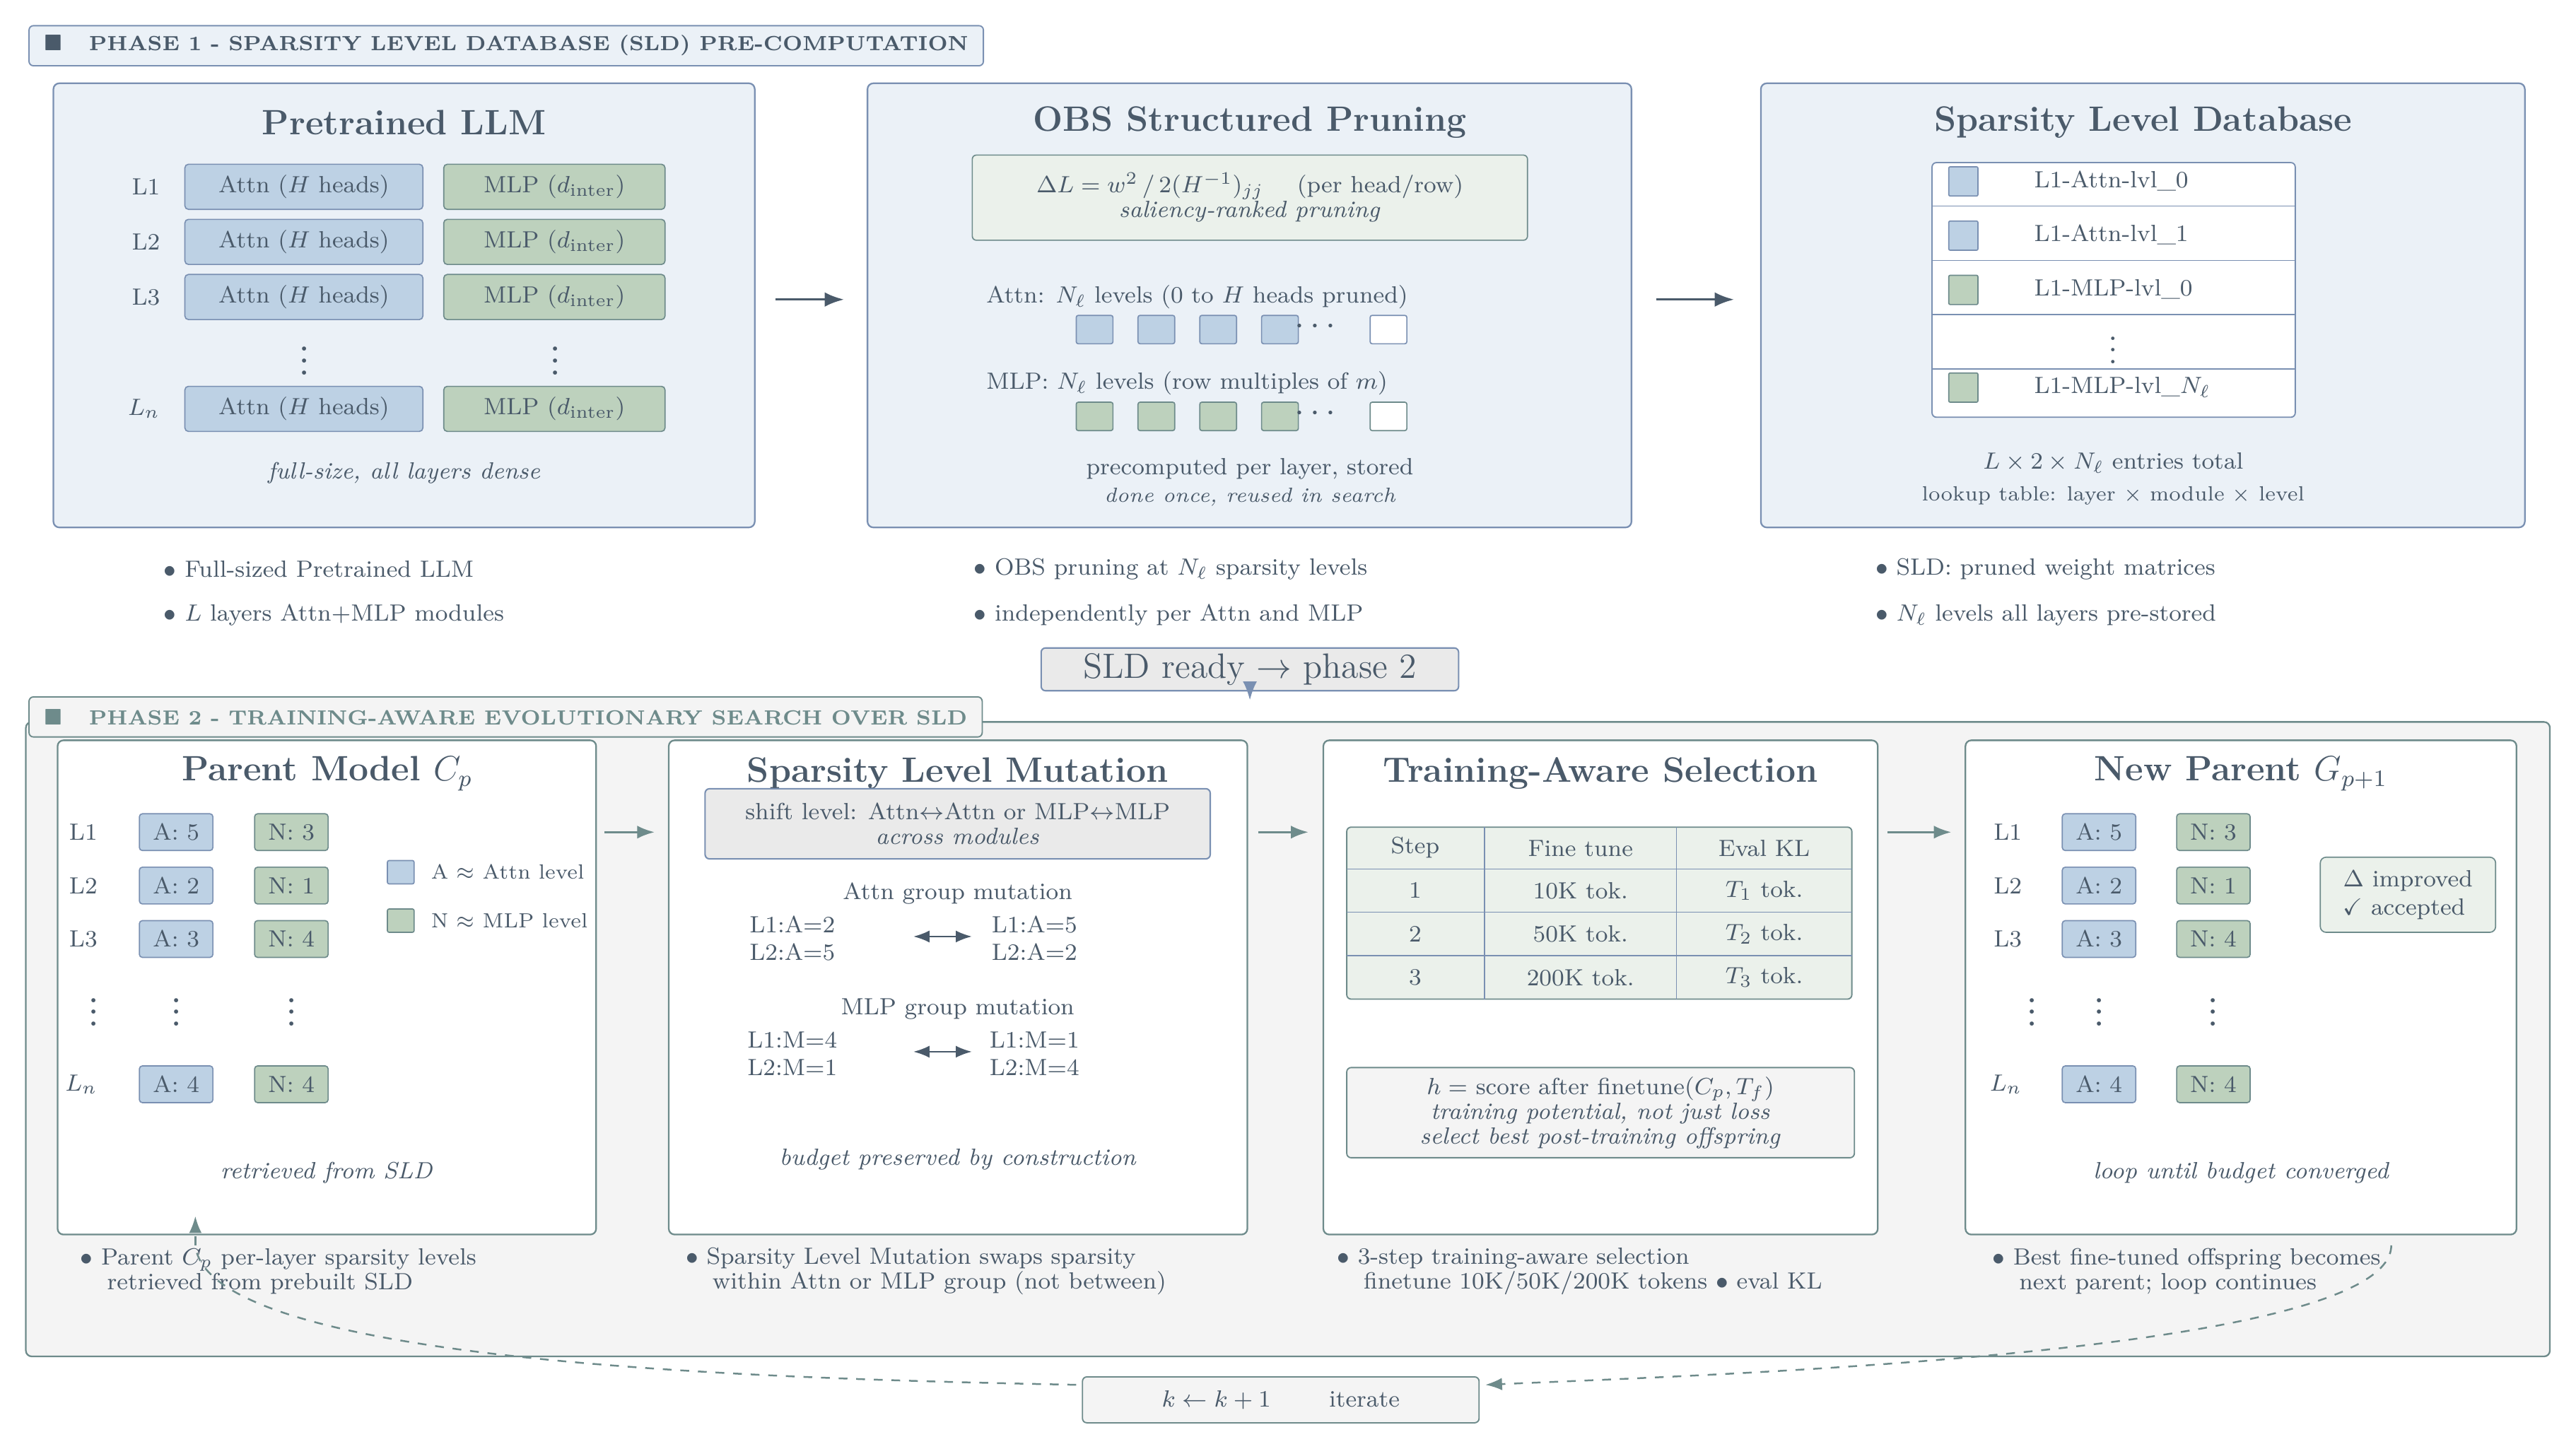
\includegraphics[width=0.94\linewidth,height=0.50\textheight,keepaspectratio]{figures/compression/darwinlm_search_loop.png}
\caption{DarwinLM search loop \citep{darwinlm2025}. The method first builds a sparsity-level database with OBS-style structured pruning, then performs training-aware evolutionary selection over stitched candidate models.}
\label{fig:darwinlm_pruning_flow}
\end{figure}

\FloatBarrier

Table~\ref{tab:preparation_cost_profile} compares the practical preparation cost of the reviewed families. This table is included separately from the empirical results because a method can report strong accuracy while still requiring a substantially different calibration, recovery, benchmarking, or search budget.

\begin{table}[H]
	\centering
	\caption{Preparation cost and evaluation requirements of representative pruning methods. The table separates low-cost post-training scoring, training-dependent structured pruning, curvature-based reconstruction, and population-based search.}
	\label{tab:preparation_cost_profile}
	\begin{tabularx}{\textwidth}{@{}>{\raggedright\arraybackslash}p{2.6cm}LL@{}}
		\toprule
		\textbf{Method} & \textbf{Dominant preprocessing cost} & \textbf{Additional requirement} \\ \midrule
		Magnitude & Linear scan $O(|W|)$ & None \\
		Wanda & Activation collection and linear scoring & Small calibration set ($\approx$128 samples) \\
		CoFi & Multi-epoch joint mask and weight optimization & Task-specific teacher; $\approx$33 h for MNLI \\
		LLM-Pruner & Forward/backward scoring over dependency groups & LoRA recovery ($\approx$2.5 h on RTX 4090) \\
		SparseGPT & Block-wise Hessian estimation and reconstruction & Calibration Hessian \\
		MRP & Group-wise mask search and compensation & Block curvature updates for N:M groups \\
		Fast PTPF & Diagonal or block Fisher estimation with mask tuning & Calibration set; optional latency lookup table \\
		ZipLM & Layer-wise Hessian updates and runtime-table search & Calibration set plus hardware benchmarking pass \\
		EvoPress / DarwinLM & Population search over compression profiles & 1--6 GPU-hours; SLD pre-computation for DarwinLM \\ \bottomrule
	\end{tabularx}
\end{table}

After the main method families have been described, the next step is to compare what they actually report. The empirical results below are therefore organized by pruning regime rather than by derivation, because perplexity, task accuracy, speedup, and recovery cost are not interchangeable measurements.

\subsection{Empirical Comparison}
\label{subsec:empirical_comparison}

The empirical evidence is organized by pruning regime. This avoids treating incompatible measurements as if they were directly comparable: unstructured and N:M methods mainly report perplexity under weight sparsity, structured methods report task accuracy or speedup after architectural removal, and search-based methods report the quality of full pruning configurations under budget constraints.

\subsubsection{Unstructured and Semi-Structured Results}

Table~\ref{tab:unsupported_comparison} keeps representative low, medium, and large model settings rather than listing every available row. The unstructured rows compare magnitude pruning, SparseGPT, and Wanda at 50\% sparsity, while the 2:4 rows show the semi-structured regime that motivates group-aware compensation such as MRP.

\begin{table}[H]
	\centering
	\caption{Representative unstructured and semi-structured pruning results on WikiText perplexity. PPL denotes perplexity; lower is better.}
	\label{tab:unsupported_comparison}
	\begin{tabular}{@{}llcccc@{}}
		\toprule
		\textbf{Model} & \textbf{Setting} & \textbf{Dense PPL} & \textbf{Magnitude PPL} & \textbf{SparseGPT PPL} & \textbf{Wanda PPL} \\
		\midrule
		LLaMA-7B  & 50\% unstructured & 5.68 & 17.29 & 7.22 & 7.26 \\
		LLaMA-30B & 50\% unstructured & 4.77 & 7.54  & 5.31 & 5.24 \\
		LLaMA-65B & 50\% unstructured & 3.56 & 5.90  & 4.57 & 4.57 \\
		\midrule
		OPT-13B   & 50\% unstructured & 10.13 & $1.2{\times}10^4$ & 11.17 & -- \\
		OPT-175B  & 50\% unstructured & 8.35  & $4.3{\times}10^4$ & 8.21  & -- \\
		\midrule
		OPT-13B   & 2:4 semi-structured & 10.13 & -- & 12.96 & -- \\
		OPT-66B   & 2:4 semi-structured & 9.34  & -- & 10.09 & -- \\
		OPT-175B  & 2:4 semi-structured & 8.35  & -- & 8.74  & -- \\
		\bottomrule
	\end{tabular}
\end{table}

The table shows two separate points. First, pure magnitude pruning can fail badly at 50\% sparsity, while activation-aware and second-order methods preserve perplexity much more effectively. Second, semi-structured 2:4 pruning remains more constrained than unconstrained unstructured pruning, so the compensation mechanism must respect the local group structure.

\subsubsection{Structured Pruning Results}

Table~\ref{tab:structured_summary} summarizes representative structured-pruning results without listing every benchmark. The rows are selected to show low, medium, and high compression or speedup regimes where available, while keeping the evaluation suite explicit: CoFi is reported on GLUE tasks and SQuADv1, Fast PTPF reports GLUE/SQuAD results, and ZipLM reports GLUE-style classification tasks as well as SQuADv1.

\begin{table}[H]
	\centering
	\caption{Representative structured Transformer pruning results across recovery regimes. GLUE denotes the General Language Understanding Evaluation benchmark, SQuADv1 denotes Stanford Question Answering Dataset version 1.1, acc. denotes accuracy, and F1 denotes question-answering F1 score.}
	\label{tab:structured_summary}
	\begin{tabular}{@{}llp{4.4cm}p{4.7cm}@{}}
		\toprule
		\textbf{Method} & \textbf{Model} & \textbf{Setting} & \textbf{Key result} \\
		\midrule
		LLM-Pruner \cite{ma2023llmpruner}
		  & LLaMA-7B & 20\% prune ratio & 98.6\% zero-shot accuracy retention after LoRA recovery \\
		  & LLaMA-7B & 50\% prune ratio & 83.6\% zero-shot accuracy retention after LoRA recovery \\
		\midrule
		CoFi \cite{xia2022structured}
		  & BERT Base & GLUE/MNLI, $\approx 12{\times}$ speedup & 80.6 acc. versus 78.8 for TinyBERT$_4$ at similar speedup \\
		  & BERT Base & SQuADv1, $\approx 8.7{\times}$ speedup & 82.6 F1, matching TinyBERT$_4$ at comparable speedup \\
		\midrule
		Fast PTPF \cite{kwon2022fast}
		  & BERT Base & GLUE and SQuADv1, FLOPs-constrained pruning & 60--70\% FLOPs with $\leq 1\%$ accuracy/F1 drop \\
		  & BERT Base & GLUE and SQuADv1, latency-constrained pruning on V100 & $1.34{\times}$--$1.47{\times}$ geometric-mean speedup depending on batch size \\
		\midrule
		ZipLM \cite{kurtic2023ziplm}
		  & BERT Base & GLUE/QNLI and MNLI, $2{\times}$ speedup & 91.4 / 84.8 acc.; essentially dense-level performance \\
		  & BERT Base & GLUE/QNLI and MNLI, $10{\times}$ speedup & 88.6 / 82.7 acc.; approximately 5M parameters \\
		  & BERT Large & SQuADv1, $10{\times}$ speedup & 89.1 F1 with 20.9M parameters \\
		\bottomrule
	\end{tabular}
\end{table}

The structured results are closer to deployment because they remove executable units, but they are also harder to compare directly. GLUE classification tasks and SQuADv1 question answering measure different behavior, and the recovery protocols also differ: CoFi uses task-specific training, LLM-Pruner depends on LoRA recovery, Fast PTPF is largely post-training, and ZipLM adds device-specific runtime profiling.

\subsubsection{Evolutionary and Search-Based Results}

Table~\ref{tab:search_summary} keeps representative search-based results and includes both EvoPress and DarwinLM. EvoPress illustrates configuration search for depth pruning and sparsity allocation, while DarwinLM shows structured evolutionary pruning with training-aware offspring selection.

\begin{table}[H]
	\centering
	\caption{Representative search-based pruning results. Wiki2 and C4 are perplexity values where lower is better; task average is accuracy where higher is better.}
	\label{tab:search_summary}
	\begin{tabular}{@{}llllccc@{}}
		\toprule
		\textbf{Setting} & \textbf{Model} & \textbf{Budget} & \textbf{Method} & \textbf{Wiki2$\downarrow$} & \textbf{C4$\downarrow$} & \textbf{Task Avg.$\uparrow$} \\
		\midrule
		Depth pruning
		  & Mistral-7B & 25\% & EvoPress & \textbf{8.66} & \textbf{12.04} & -- \\
		  & Mistral-7B & 25\% & ShortGPT & 43.26 & 40.16 & -- \\
		  & Mistral-7B & 25\% & Shortened LLaMA & 14.94 & 19.30 & -- \\
		\midrule
		Depth pruning
		  & Llama-2-7B & 37.5\% & EvoPress & \textbf{17.98} & \textbf{18.91} & -- \\
		  & Llama-2-7B & 37.5\% & ShortGPT & 70.94 & 63.51 & -- \\
		  & Llama-2-7B & 37.5\% & Shortened LLaMA & 35.37 & 26.07 & -- \\
		\midrule
		Unstructured allocation
		  & Mistral-7B & 70\% & EvoPress & \textbf{14.42} & \textbf{16.46} & \textbf{53.8} \\
		  & Mistral-7B & 70\% & OWL & 17.22 & 21.66 & 51.9 \\
		  & Mistral-7B & 70\% & Uniform & 23.08 & 30.03 & 49.9 \\
		\midrule
		Structured search
		  & Llama-2-7B & 2.7B model & DarwinLM & -- & -- & 62.8 after 10B-token post-training \\
		  & Llama-2-7B & 2.7B model & ShearedLLaMA & -- & -- & 62.6 after 50B-token post-training \\
		\bottomrule
	\end{tabular}
\end{table}

The search results support the same conclusion from two directions. EvoPress improves over local or heuristic allocation when multiple removals interact, and DarwinLM shows that training-aware evolutionary selection can produce stronger structured models with less post-training data than a fixed pruning baseline.

\subsubsection{Cross-Regime Synthesis}

Table~\ref{tab:pruning_empirical_summary} aggregates the evidence at a higher level. It is not meant to replace the detailed result tables above; it summarizes what each regime establishes for the design of a pruning-search method.

\begin{table}[H]
	\centering
	\caption{Aggregated interpretation of the empirical pruning evidence by regime.}
	\label{tab:pruning_empirical_summary}
	\begin{tabularx}{\textwidth}{@{}>{\raggedright\arraybackslash}p{2.5cm}>{\raggedright\arraybackslash}p{3.0cm}LL@{}}
		\toprule
		\textbf{Regime} & \textbf{Representative setting} & \textbf{Selected evidence} & \textbf{Reading} \\
		\midrule
		Weight-level unstructured
		& LLaMA-7B, 50\% sparsity
		& Dense PPL 5.68; magnitude 17.29; SparseGPT 7.22; Wanda 7.26.
		& Better saliency preserves perplexity, but the resulting pattern remains unstructured and does not guarantee dense-kernel speedup. \\
		\addlinespace
		Semi-structured N:M
		& OPT-13B, 2:4 sparsity
		& Dense PPL 10.13; SparseGPT-style compensation gives 12.96 under the 2:4 constraint.
		& N:M sparsity needs group-aware compensation, which motivates MRP-style joint treatment of simultaneously removed weights. \\
		\addlinespace
		Structured LLM pruning
		& LLM-Pruner on LLaMA-7B
		& 20\% prune ratio retains 98.6\% zero-shot accuracy after LoRA recovery; 50\% retains 83.6\%.
		& Dependency-aware pruning keeps the model executable, but the final quality depends strongly on recovery. \\
		\addlinespace
		Structured encoder pruning
		& CoFi, Fast PTPF, and ZipLM on BERT
		& CoFi reaches 80.6 MNLI acc. near $12{\times}$ speedup; Fast PTPF keeps 60--70\% FLOPs with $\leq$1\% drop; ZipLM reaches 88.6/82.7 QNLI/MNLI acc. at $10{\times}$ speedup.
		& Structured pruning can produce executable acceleration, but the protocols differ in training cost, hardware profiling, and recovery budget. \\
		\addlinespace
		Search-based pruning
		& EvoPress and DarwinLM
		& EvoPress improves depth-pruning and sparsity-allocation baselines; DarwinLM reports 62.8 average accuracy after 10B-token post-training versus 62.6 for ShearedLLaMA after 50B tokens.
		& Configuration search addresses global allocation, while training-aware selection improves structured candidates beyond one-shot scoring. \\
		\bottomrule
	\end{tabularx}
\end{table}
